\documentclass[UTF8,a4paper,12pt]{ctexart}

\usepackage[margin=2.4cm]{geometry}
\usepackage{amsmath}
\usepackage{graphicx}
\usepackage{booktabs}
\usepackage{multirow}
\usepackage{array}
\usepackage{float}
\usepackage{caption}
\usepackage{etoolbox}
\usepackage[hidelinks]{hyperref}
\hypersetup{pdftitle={光电、红外测距与灰度传感器特性测试实验报告}, pdfsubject={传感器实验}, pdfcreator={}}
\usepackage{enumitem}

\captionsetup{font=small,labelsep=quad,skip=4pt}
\AtBeginEnvironment{table}{\small}
\captionsetup[table]{position=top}
\captionsetup[figure]{position=bottom}
\renewcommand{\arraystretch}{1.08}
\linespread{1.2}
\setlength{\parskip}{1pt}
\raggedbottom
\renewcommand{\topfraction}{0.92}
\renewcommand{\bottomfraction}{0.85}
\renewcommand{\textfraction}{0.08}
\renewcommand{\floatpagefraction}{0.9}
\setcounter{topnumber}{3}
\setcounter{bottomnumber}{2}
\setcounter{totalnumber}{5}
\pagestyle{plain}
\setlist[enumerate]{itemsep=2pt,topsep=4pt,parsep=0pt,leftmargin=2.2em}
\setlist[itemize]{itemsep=2pt,topsep=4pt,parsep=0pt,leftmargin=2.2em}

\title{光电、红外测距与灰度传感器\\特性测试实验报告}
\author{}

\begin{document}

\begin{center}
{\LARGE\bfseries 光电、红外测距与灰度传感器}\\[6pt]
{\LARGE\bfseries 特性测试实验报告}\\[18pt]
{\zihao{5}
小组成员：韩颂义、陈盈皓、张雨童\\[4pt]
学号：\underline{\hspace{3.0cm}}\quad 实验日期：2026 年 10 月 26 日}
\end{center}

\vspace{1.2em}


\section{光电传感器}
\subsection{实验方法}
以粗糙表面和光面为目标，分别记录去程和回程的触发位置，各测量三次。调整目标夹角至 $15^{\circ}$、$30^{\circ}$、$45^{\circ}$、$60^{\circ}$，每个角度测量三次。

\subsection{原始数据}
表中探测距离为尺上读数减去传感器末端位置 3.5 cm 后的数值。

\begin{table}[H]
  \centering
  \caption{不同反光表面的探测距离}
  \label{tab:photo-surface}
  \begin{tabular}{cccc}
    \toprule
    表面 & 次数 & 去程/cm & 回程/cm \\
    \midrule
    \multirow{3}{*}{粗糙} & 1 & 36.1 & 35.9 \\
     & 2 & 35.8 & 35.7 \\
     & 3 & 36.3 & 36.0 \\
    \midrule
    \multirow{3}{*}{光面} & 1 & 52.2 & 51.5 \\
     & 2 & 51.5 & 54.0 \\
     & 3 & 53.0 & 49.9 \\
    \bottomrule
  \end{tabular}
\end{table}

\begin{table}[H]
  \centering
  \caption{不同目标夹角的探测距离}
  \label{tab:photo-angle}
  \begin{tabular}{cccc}
    \toprule
    角度/$({}^{\circ})$ & 第 1 次/cm & 第 2 次/cm & 第 3 次/cm \\
    \midrule
    15 & 33.3 & 33.8 & 33.9 \\
    30 & 30.0 & 30.0 & 30.1 \\
    45 & 27.7 & 27.8 & 27.4 \\
    60 & 23.9 & 24.4 & 24.4 \\
    \bottomrule
  \end{tabular}
\end{table}

\section{红外测距传感器}
\subsection{实验方法}
静态实验在 10～80 cm 范围内每隔 10 cm 记录 ADC 值，分别测量白色、黑色目标及不同夹角的目标。动态实验让滑台以 25、50、100、200 圈/分将目标从 80 cm 移向 10 cm，同时记录 ADC 值和时间。

\subsection{原始数据}
静态基准记录中的目标颜色和夹角未注明。

\begin{table}[H]
  \centering
  \caption{静态基准 ADC 值}
  \label{tab:distance-static}
  \begin{tabular}{cc}
    \toprule
    距离/cm & ADC 值 \\
    \midrule
    10 & 2593.30 \\
    20 & 1323.50 \\
    30 & 859.45 \\
    40 & 628.25 \\
    50 & 489.50 \\
    60 & 400.50 \\
    70 & 325.20 \\
    80 & 276.80 \\
    \bottomrule
  \end{tabular}
\end{table}

\begin{table}[H]
  \centering
  \caption{不同目标颜色的 ADC 值}
  \label{tab:distance-color}
  \begin{tabular}{ccc}
    \toprule
    距离/cm & 白色 & 黑色 \\
    \midrule
    10 & 2589.85 & 2601.20 \\
    20 & 1325.40 & 1288.45 \\
    30 & 881.70 & 869.95 \\
    40 & 640.35 & 627.55 \\
    50 & 521.85 & 493.30 \\
    60 & 404.45 & 393.55 \\
    70 & 318.50 & 306.30 \\
    80 & 275.00 & 247.50 \\
    \bottomrule
  \end{tabular}
\end{table}

\begin{table}[H]
  \centering
  \caption{不同目标夹角的 ADC 值}
  \label{tab:distance-angle}
  \begin{tabular}{cccc}
    \toprule
    距离/cm & $15^{\circ}$ & $30^{\circ}$ & $45^{\circ}$ \\
    \midrule
    10 & 2595.80 & 2585.95 & 2423.80 \\
    20 & 1296.95 & 1235.60 & 1197.20 \\
    30 & 847.25 & 820.70 & 815.15 \\
    40 & 624.40 & 597.95 & 591.05 \\
    50 & 515.15 & 464.80 & 464.65 \\
    60 & 410.30 & 393.85 & 355.90 \\
    70 & 317.80 & 302.25 & 302.15 \\
    80 & 260.85 & 283.10 & 264.25 \\
    \bottomrule
  \end{tabular}
\end{table}

\begin{figure}[H]
  \centering
  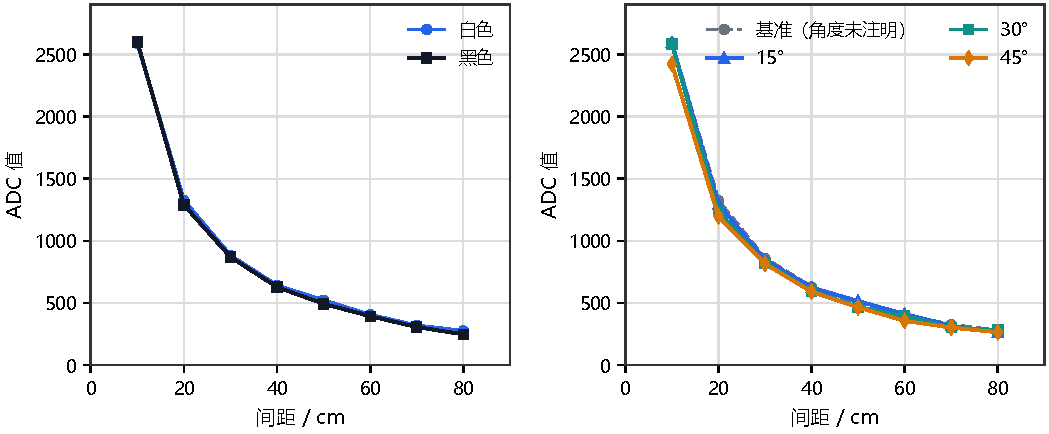
\includegraphics[width=0.95\textwidth]{figures/fig_distance_color_angle.pdf}
  \caption{不同目标颜色和夹角下的 ADC 数据}
\end{figure}

\begin{table}[H]
  \centering
  \caption{动态实验条件}
  \begin{tabular}{cccc}
    \toprule
    速度/(圈/分) & 时长/s & 标称速度/(cm/s) & 窗口跨度/cm \\
    \midrule
    25  & 22.448 & 3.125 & 0.65 \\
    50  & 11.229 & 6.25  & 1.28 \\
    100 & 5.759  & 12.5  & 2.52 \\
    200 & 2.895  & 25.0  & 4.98 \\
    \bottomrule
  \end{tabular}

  \vspace{2pt}
  \parbox{0.92\linewidth}{\small 注：标称速度按 200 圈/分约为 25 cm/s 等比估算；窗口跨度为 5 点滤波窗口对应的距离跨度。}
\end{table}

动态实验分别采用 25、50、100、200 圈/分四种滑台速度。

对运动区间的 ADC 数据采用离线居中 5 点中值滤波：取当前点及前后各 2 点的中值，边界处重复端点值。

\begin{figure}[H]
  \centering
  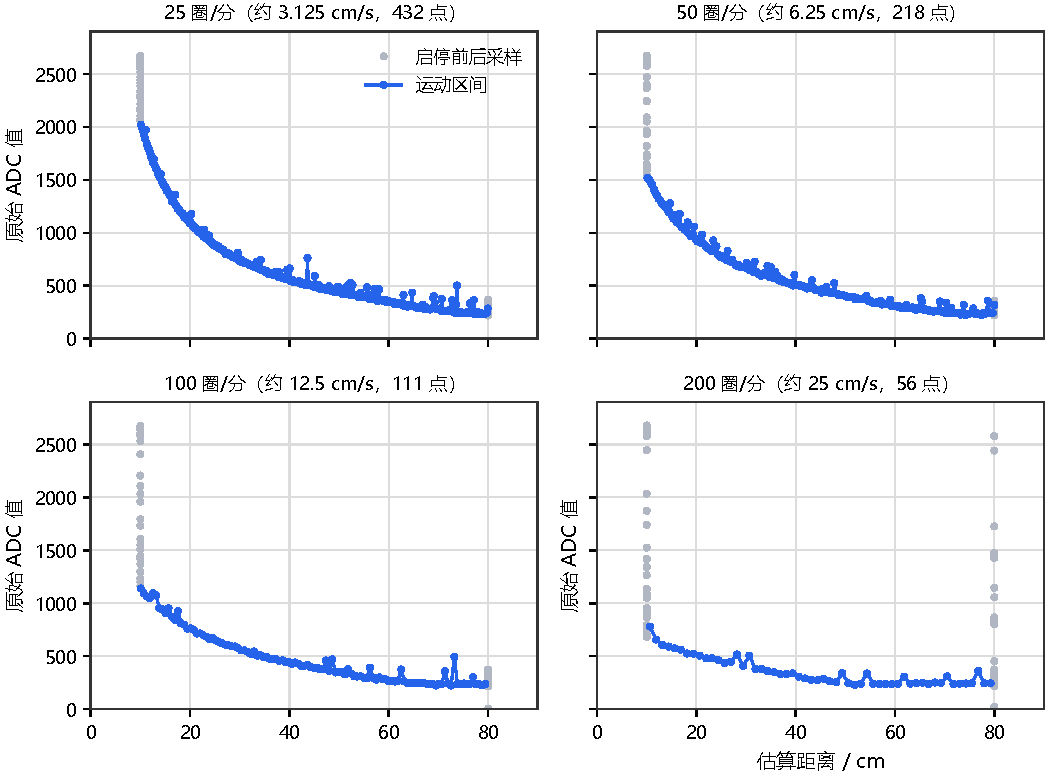
\includegraphics[width=0.64\textwidth]{figures/fig_dynamic_raw.pdf}
  \caption{四种滑台速度下的原始 ADC 与估算距离}
  \label{fig:dynamic-raw}
\end{figure}

\begin{figure}[H]
  \centering
  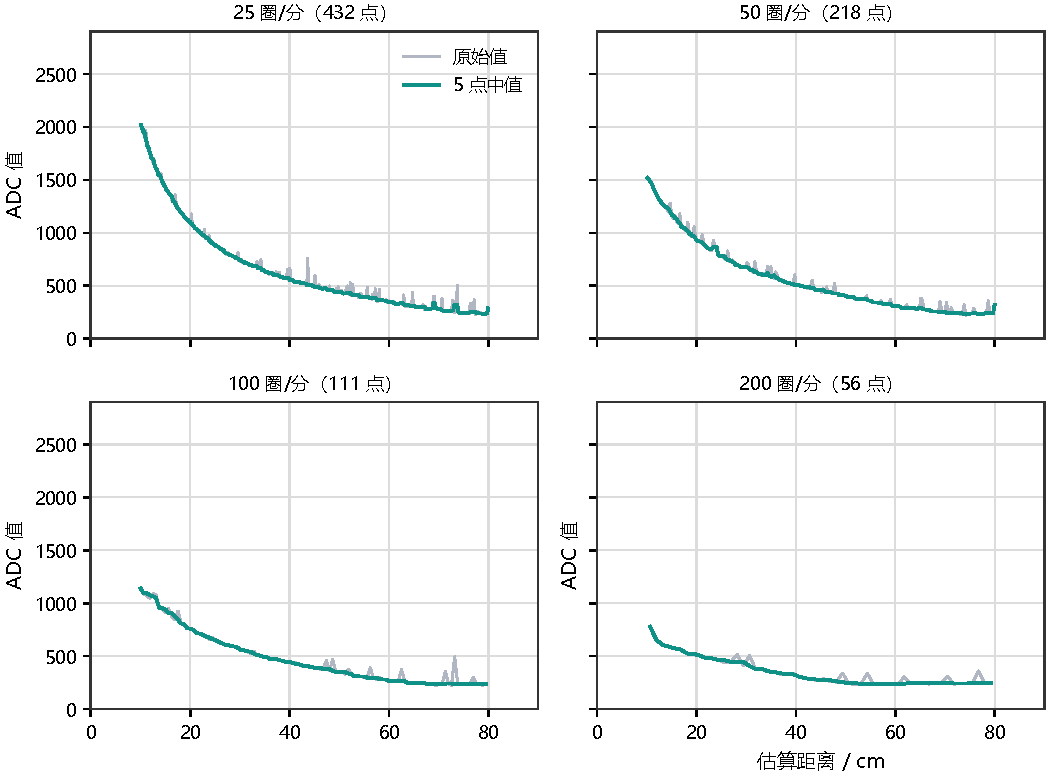
\includegraphics[width=0.64\textwidth]{figures/fig_dynamic_filtered.pdf}
  \caption{四种滑台速度下的原始数据与 5 点中值滤波结果}
  \label{fig:dynamic-filtered}
\end{figure}

\section{灰度传感器}
\subsection{实验方法}
在 1、3、5、15 cm 四种距离下，分别记录 1～9 号灰度色卡的 ADC 值；在 3 cm 距离下，分别记录暗、亮两种环境条件下的 ADC 值。1 号最白，9 号最黑。

\subsection{原始数据}
\begin{table}[H]
  \centering
  \caption{不同距离和色卡的 ADC 值}
  \label{tab:gray-distance}
  \begin{tabular}{ccccc}
    \toprule
    色卡编号 & 1 cm & 3 cm & 5 cm & 15 cm \\
    \midrule
    1（最白） & 2450 & 1280 & 455 & 125 \\
    2 & 2050 & 1000 & 355 & 125 \\
    3 & 1350 & 880 & 290 & 110 \\
    4 & 930 & 640 & 243 & 96 \\
    5 & 630 & 460 & 200 & 85 \\
    6 & 535 & 335 & 150 & 80 \\
    7 & 380 & 245 & 123 & 68 \\
    8 & 270 & 150 & 90 & 65 \\
    9（最黑） & 185 & 113 & 80 & 65 \\
    \bottomrule
  \end{tabular}
\end{table}

\begin{figure}[H]
  \centering
  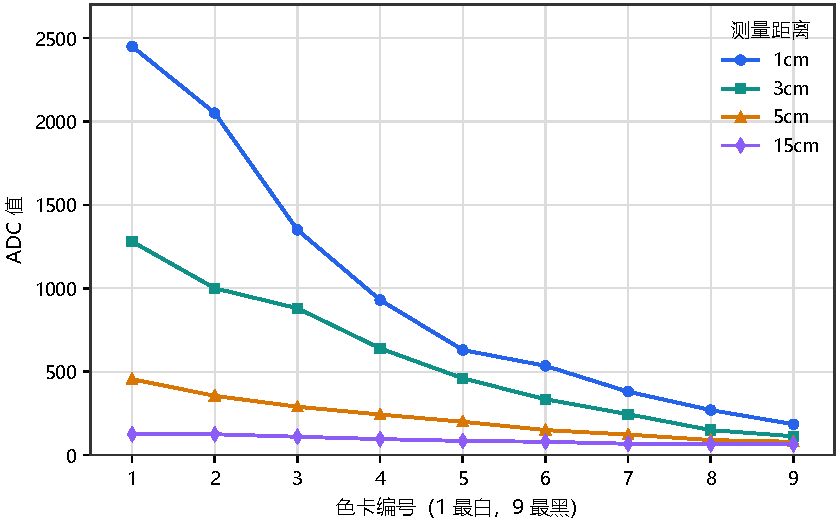
\includegraphics[width=0.74\textwidth]{figures/fig_gray_cards.pdf}
  \caption{不同距离和色卡的 ADC 数据}
\end{figure}

\begin{table}[H]
  \centering
  \caption{3 cm 距离下不同光照条件的 ADC 值}
  \label{tab:gray-light}
  \begin{tabular}{ccc}
    \toprule
    色卡编号 & 暗 & 亮 \\
    \midrule
    1 & 1256 & 1760 \\
    2 & 959 & 1347 \\
    3 & 748 & 1069 \\
    4 & 554 & 774 \\
    5 & 419 & 578 \\
    6 & 351 & 418 \\
    7 & 263 & 270 \\
    8 & 218 & 204 \\
    9 & 175 & 148 \\
    \bottomrule
  \end{tabular}
\end{table}

\begin{figure}[H]
  \centering
  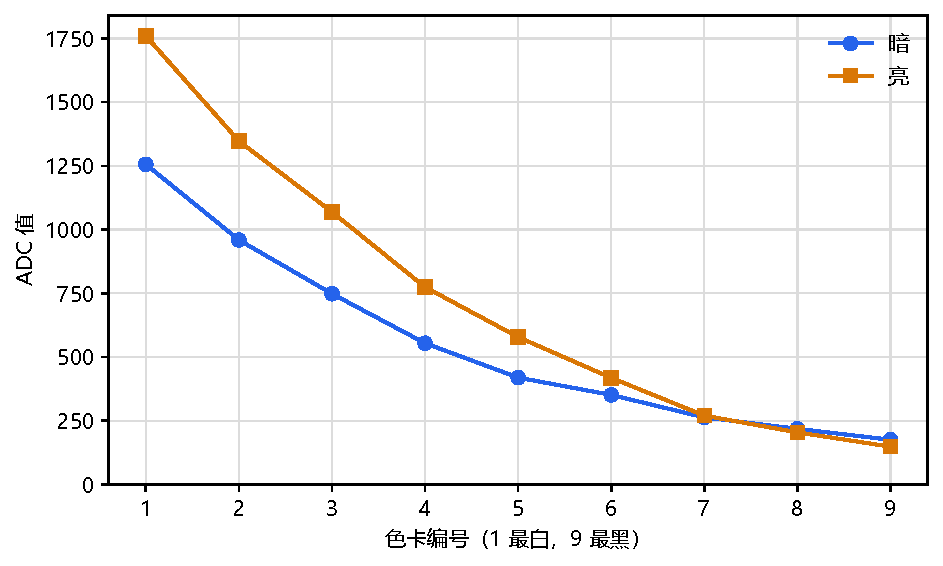
\includegraphics[width=0.74\textwidth]{figures/fig_gray_light_raw.pdf}
  \caption{3 cm 距离下不同光照条件的 ADC 数据}
\end{figure}

\end{document}
